 
\documentclass[a4paper,12pt]{diplom}
% \usepackage[latin1]{inputenc}
% \usepackage[utf8]{inputenc}
\inputencoding{utf8} % Кодировка вашего файла


\usepackage{paratype} % Шрифты (можно отключить, если дает ошибку)
%% Немного увеличим шрифт в математическом режиме, чтобы соответствовать размерам Paratype-шрифтов
\DeclareMathSizes{12}{13.4}{11}{10}

\usepackage[left=3cm,right=2cm,top=2cm,bottom=2cm]{geometry} % Размеры полей
\usepackage[onehalfspacing]{setspace} % Полуторный интервал
%\renewcommand{\baselinestretch}{1.25} % Полуторный интервал
\usepackage{indentfirst} % Абзацный отступ в начале разделов
\setlength{\parindent}{1.25cm} % Величина абзацного отступа

\usepackage[pdftex]{graphicx} % Для вставки изображений
\usepackage{array} % Для таблиц
\usepackage{booktabs} % Для красивых таблиц 
\usepackage{tikz} % Рисунки с помощью TikZ
\usepackage[linesnumbered,lined,ruled]{algorithm2e} % Для оформления псевдокода
%\usepackage{algorithm} % Альтернатива оформления псевдокода
%\usepackage{algpseudocode} % Альтернатива оформления псевдокода
\usepackage{listings} % Оформление листингов программ
\usepackage{icomma} % Удаляем тонкий пробел после запятой в мат. режиме

% Если на нумерованную формулу нет ссылки в тексте,
\mathtoolsset{showonlyrefs} % то она становится ненумерованной

% microtype улучшает распределение символов в строке
\usepackage{microtype}  % Можно отключить, если возникают ошибки компиляции

% Формируем PDF с полноценными перекрестными ссылками
\usepackage[unicode, pdfborder={0 0 0}, pdfstartview=FitV]{hyperref}

\usepackage{listingsutf8}

% Часто используемые макросы
\newcommand{\N}{\mathbb{N}}  % Множество натуральных чисел
\newcommand{\Z}{\mathbb{Z}}  % Множество целых чисел
\newcommand{\R}{\mathbb{R}}  % Множество действительных чисел
\DeclareMathOperator{\sgn}{sgn} % Знак числа
\DeclareMathOperator{\M}{\mathsf{M}} % Матожидание
\newcommand{\from}{\colon} % Двоеточие в определении функции. Пример: $f \from \R \to \N$.
% Заменяем англоязычные обозначения на русские
\renewcommand{\le}{\leqslant}
\renewcommand{\leq}{\leqslant}
\renewcommand{\ge}{\geqslant}
\renewcommand{\geq}{\geqslant}
\renewcommand{\emptyset}{\varnothing}
\renewcommand{\epsilon}{\varepsilon}


%%%%%%%%%%%%%%%%%%%%%%%%%%
% Конец преамбулы
%%%%%%%%%%%%%%%%%%%%%%%%%%

\begin{document}

% Содержимое титульного листа

%\LetterHead{Минобр...}
\Kafedra{Кафедра компьютерных сетей}

% Зав. кафедрой
\ZavKaf{Заведующий кафедрой, \\д.ф.-м.н., профессор}{С.\,Д.~Глызин}
% Если это курсовая работа и виза зав. каф. не нужна, раскомментируйте следующую строку
%\Kursovaya

% Вид работы: Курсовая работа, Выпускная квалификационная работа, 
\DocumentType{\large Выпускная квалификационная работа}

% Название дипломной работы
\Title{\begin{Large}\bfseries Разработка инструмента экспорта \\ данных моделей в формате XML\end{Large}}

% Направление подготовки
\Napr{по направлению\\ 02.03.02 Прикладная математика и информатика}

% Руководитель
\Chief{Научный руководитель\\ к.ф.-м.н., доцент}{И.\,В.~Парамонов}

% Автор
\Author{Студент группы ИВТ-42БО}{М.\,А.~Лавров}

%\City{Ярославль}
%\Year{2017}


% Создаем титульный лист
\maketitle
\chapternonum{Реферат}

Объем \total{page} с., \total{chapternum} гл., 10 рис.,
\total{tablenum} табл., \total{bibnum} источников, \total{appnum} прил.

\medskip

Ключевые слова: \textbf{XML, Java, Java EE, Java Nashorn, StAX, веб-приложения, процесс разработки ПО.}

В данной работе будет описан инструмент экспорта данных моделей в XML формат, реализация взаимодействия пользователя с настройками инструмента, а также его применимость в проекте АСП ФК.

Цель работы: Разработать настраиваемый инструмент для экспорта данных моделей по спецификациям заказчика.

В процессе работы было изучено строение интерфейсов проекта АСП ФК, изучен принцип работы сервлетов в Java EE и изучены различные принципы построения XML-документов.

В результате работы были разработаны инструмент экспорта и интерфейс взаимодействия с ним.

\medskip

% Содержание
\tableofcontents[Содержание]

% Пример ненумерованной главы
\chapternonum{Введение}

В настоящее время информационные технологии занимают все более важное место в жизни общества. С развитием компьютерных технологий возникает необходимость в создании программных инструментов, которые бы позволяли упростить и автоматизировать процессы обработки и передачи данных. Одним из таких инструментов является формат XML, который позволяет описывать структуру и содержание документов. XML широко используется для хранения и передачи данных в различных областях, таких как настольные и веб-приложения, научные исследования и многие другие.

Цель моей выпускной квалификационной работы -- разработка инструмента экспорта данных моделей в формате XML, поддерживающего настройку отображения данных из моделей.

Разработанный инструмент может быть использовал для настройки XML-представления моделей в разных системах, которые используются Казначейством России.

\chapter{Обзор предметной области}

\section{Описание проекта, в рамках которого был разработан инструмент}

Инструмент реализуется в рамках проекта АСП ФК (Автоматизированная система планирования Федерального Казначейства). Он предназначен для автоматизации осуществления проверки казначейством России объектов контроля. Сначала эти проверки планируются -- для этого предназначен блок планирования в проекте. Базовый интерфейс данного блока -- План-график (таблица). После того как проверка была спланирована, ее нужно исполнить, т.е. провести. Тут базовых интерфейса 2: Паспорт КМ [реестр] и Паспорт АП [реестр], где КМ -- контрольное мероприятие, а АП -- административное производство. Реализованный проект позволяет распределять нагрузку между сотрудниками ФК, упрощает взаимодействие между подразделениями, позволяет просматривать и использовать информацию из внешних систем, а также формировать печатные документы и отчёты на основе электронных данных.

\section{Описание формата XML}

XML (Extensible Markup Language) -- это формат данных, который используется для обмена информацией между компьютерами \cite{W3C:XML}. Он был создан в 1998 году и является расширяемым, то есть может быть адаптирован под различные задачи и потребности.

XML представляет собой текстовый файл, состоящий из элементов (тегов), атрибутов и значений. Каждый элемент начинается с открывающего тега, в котором указывается имя элемента, а также, опционально, атрибуты и его пространство имён, и заканчивается закрывающим тегом с тем же именем и пространством имён, если таковое задано у открывающего. Между открывающим и закрывающим тегами может находиться другой XML-код, включая другие элементы, атрибуты и значения.

Атрибуты используются для передачи дополнительной информации, которая относится к элементу. Они указываются в открывающем теге и могут содержать любые данные, включая текст, числа и ссылки.

Значения элементов могут быть как текстовыми, так и числовыми, а также могут содержать ссылки на другие элементы или файлы.

XML имеет много преимуществ перед другими форматами данных. Он является универсальным, расширяемым и легко читаемым компьютерами и человеком. Он также может быть использован для передачи данных между различными платформами и языками программирования.

\section{Описание моделей данных}

Модель данных представляет собой набор вычислимых и хранимых полей. Каждое поле задаётся методом с названием вида \textbf{get + название поля}. Далее, если поле хранимое, необходимо указать аннотацию \textbf{@Column} и параметром \textbf{name} в ней задать строковое значение -- название колонки. Если поле вычислимое, то нужно только указать аннотацию \textbf{@Transient}. Также есть возможно задания полей с помощью SQL формул аннотацией \textbf{@Formula} или задачей получения значения с помощью операций над экземпляром модели.  Если поле изменяемо, то ниже после метода \textit{get} указывается ещё и метод вида \textbf{set + название поля}. Иначе, поле будет константным и поменять его можно будет разве что через запрос к базе данных. Каждая модель имеет поле идентификатора. Для него гарантируется уникальности в отображаемой таблице.

Также, с помощью множественной имплементации (реализации) можно добавлять в модель данных дополнительное поведение. С помощью такого инструмента можно обобщать модели на разных уровнях абстракции.

Каждая модель при старте приложения преобразуется в таблицу в базе данных средствами Hibernate.

\section{Описание типичного интерфейса в проекте}

Интерфейс в проекте представляет собой веб-страницу. Внутри неё есть табличного вида дополнительные страницы, как главный элемент и панель кнопок сверху. В таблице есть некоторые перечень записей, между которыми можно переключаться кликом мышки. Первая кнопка на этой панели открывает дополнительную панель снизу с детализациями записи в главной таблице. Преимущественно они служат для заполнения полей в модели базовой таблице, которые сами являются либо моделями, либо же списками моделей. Например, мероприятие, как модель главной таблицы, и периоды проведения как детализация.

\section{Обзор используемых технологий}

Сам проект постоен на Java EE (Java Enterprise Edition) - это платформа для разработки и выполнения корпоративных приложений на языке Java \cite{Argun:2014}. Она предоставляет набор API и инструментов для создания масштабируемых, надежных и безопасных приложений, которые могут быть запущены на различных серверах приложений.

Соответственно, внутри проекта используется язык Java 1.8 \cite{Shildt:2018}.

Для работы инструмента используется сервлет -- это одна из внутренних технологий Java EE. Она используется для создания обработки запросов от пользователей.

В проекте используется СУБД PostgreSQL. Она производительна и у неё достаточно обширный синтаксис. Также, ею поддерживается множество расширений (Extensions).

Для связи моделей с таблицами в базе данных используется Hibernate - это фреймворк для объектно-реляционного отображения (ORM) в Java. Он предоставляет инструменты для работы с базами данных, которые позволяют разработчикам работать с базами данных на более высоком уровне абстракции, используя объекты Java вместо SQL-запросов. Описание таблиц в базе данных с помощью этого фреймворка является намного более понятным для человека. Одним из неоспоримых плюсов данного фреймворка являются возможности создавать ссылки на другие модели, инструментами фреймворка и задавать отношения <<Один ко многим>>, <<Многие ко многим>> и <<Один к одному>> между моделями данных. Это позволяет разработчику тратить на много меньше времени на создание моделей данных.

Для задания фиксированных значений используется движок JavaScript Nashorn. С помощью него код на JavaScript будет компилироваться в Java-код для последующей обработки. Он доступен в стандартной поставке  Java 1.8 и заменяет устаревший Rhino. В проекте он используется в тех местах, где предполагается работа пользователя после сдачи проекта. Он крайне удобен в данном случае, его использование упростит работу людей, которые будут модифицировать проект на этапе его поддержки, так как не будет необходимости для рутинных действий разбираться с большим количеством кода на языке Java.

В качестве среды разработке используется Intellij IDEA, являющаяся как минимум одной из наиболее популярных сред для разработки на языке Java.

Также используется система контроля версий Git, дающая обширное количество инструментов для манипуляции отслеживания и манипуляций с изменениями в коде проекта.

\chapter{Анализ требований}

\section[Постановка задачи]{Постановка задачи для инструмента экспорта данных моделей в формате XML}

Необходимо создать инструмент, который бы принимал объекты, принадлежащие модели и выгружал их в виде XML-файла.  

Поддерживаемые возможности:

\begin{enumerate}[label=\arabic{enumi})]
	\item Инструмент должен быть оформлен в виде отдельного интерфейса в системе.
    \item Новые сценарии (наборы настроек такого инструмента) на существующие модели не должны затрагивать java представление самих моделей.
    \item Задания структуры элементов (тегов) XML-документа:
        \begin{itemize}
	       \item Пространство имён, которому принадлежит атрибут.
	       \item Название атрибута.
	       \item Родительский атрибут.
              \item Название колонки в источнике.
              \item Порядок.
	  \end{itemize}
    \item У каждого элемента, кроме корневого, должна быть реализована возможность задания атрибутов элемента (тега), имеющих как вычислимое значение, задающее скриптом, так и значение из набора данных.
    \item Возможность выставления фиксированного значения у выбранного атрибута, задаваемого кодом в синтаксисе JavaScript Nashorn
    \item Возможность задания элементов структур, входящих в главный элемент, но не входящий в структуру тегов, генерирующихся с помощью задания скрипта на языке JavaScript и обрабатываемого с помощью Nashorn. Например, даты создания XML-документа. Причём данные элементы также должны иметь возможно задания атрибутов с фиксированным значением.
    \item Необходима возможность вызова создания XML-документа по созданной структуре экспорта через кнопку на верхней панели интерфейса.
    \item Если значения в модели нет, или оно пустое, то необходимо опускать из описания этой экземпляра модели данных обрабатываемый элемент. Даже в случае, если атрибуты для него существуют в модели.
    \item В случае если у элементов, описанных в пункте 6 нет данных для заполнения, то выводить ошибку пользователю о некорректной структуре.
\end{enumerate}

\section{Анализ существующих инструментов на соответствие требованиям}

На данный момент для Java существует множество библиотек, для сериализации моделей. Разберём применимость их к задаче на примере самый популярных и поддерживаемых.

\begin{enumerate}[label=\arabic{enumi})]
	\item JAXB (Java Architecture for XML Binding) - библиотека, которая позволяет сериализовать и десериализовать Java-объекты в XML-документы \cite{Java:JAXP}. Является стандартной библиотекой Java, которая включена в JDK. Поддерживает работу с большими XML-документами. Данная библиотека не подойдёт нам. Название корневого элемента, порядок, сериализуемые и несериализуемые поля необходимо указывать с помощью аннотаций. Это противоречит постановки задачи в пункте 2.
 
    \item  XStream - это библиотека, которая позволяет сериализовать и десериализовать Java-объекты в XML-документы \cite{Str:XStream}. Она использует рефлексию для определения структуры объекта и может работать с объектами, которые не имеют аннотаций. Здесь нарушается также пункт 2, но уже из-за необходимости использовать аннотации для настройки <<пространств имён>>.

    \item  Jackson - это библиотека для сериализации и десериализации Java-объектов в различные форматы, в том числе в XML. Она позволяет работать с объектами в формате JSON, YAML и XML. В данном случае как минимум одна из проблем заключается в том, что без использования аннотаций нет возможности задать порядок аттрибутов. Это противоречит 3 пункту постановки задачи.

    \item  Simple XML - это библиотека, которая позволяет сериализовать и десериализовать Java-объекты в XML-документы \cite{Str:SimpleXML}. Она использует аннотации для указания параметров сериализации и десериализации и может работать с объектами, которые не имеют конструкторов по умолчанию. В данном случае необходимо менять модель, что также, как и с JAXB, противоречит 2 пункту постановки задачи.
\end{enumerate}

Существующие решения не позволяют полностью удовлетворить требованиям постановки задачи. Все они требуют использования аннотаций для реализации задачи, а значит затрагивают модели.

\chapter{Разработка инструмента}

\section{Описание способа взаимодействия с инструментом}

Инструмент будет реализован с помощью сервлета. Это удобный механизм для расширения возможностей сервера, он работает по типу <<Запрос-Ответ>>, что как раз подходит под требования и даёт возможность для быстрого изменения места вызова инструмента.

\section{Описание визуальной часть интерфейса взаимодействия с инструментом}

При создании новой записи на интерфейсе, необходимо будет задать два поля: Наименование и Код. Они нужно исключительно для удобства поиска в случае Кода и понимания применимости в случае Наименования. Такая запись в дальнейшем будет именоваться в дальнейшем <<сценарий экспорта>>.

Также будет нужно поле для Источника данных. Это внутренний инструмент, о котором будет рассказано в часть реализации.

Настройки <<структуры>> и <<пространства имён>> будет сделано с помощью детализаций. Это удобное представление полей для записи, которые можно создать прямо при создании нового сценария. 

Первая будет называться <<пространство имён>> и указывать применимые к экспортируемому XML-файлу пространства имён. Это специальный инструмент, позволяющий не допускать конфликта имён XML-элементов и их атрибутов. Они позволяют использовать названые одинаково элементы если те принадлежат к разным пространствам имён. Задать их можно как с помощью атрибута xmlns, так и с помощью тега <namespace>. В инструменте будет использован первый способ, так как он более удобен при создании документа в данном случае. Такой атрибут будет выглядеть следующим образом:

\medskip
\textbf{xmlns:Название="Путь к пространству"}
\medskip

Соответственно необходимы колонки <<тег пространства>> и <<имя пространства>>.

Вторая детализация -- <<структура>>. Она позволяет задавать структуру тегов, их отношения (родитель--потомок), порядок внутри группы потомков, а также колонки в наборе данных и скрипт для вычисления значения.

Дабы удовлетворить постановке задачи, будет реализована кнопка, при нажатии на которую выполняется генерация XML--документа и последующее его скачивание средствами браузера.

\section{Реализация визуальной части интерфейса взаимодействия с инструментом}

Для создания новых визуальных интерфейсов в проекте необходимо:

\begin{itemize}
    \item Создать класс формы
    \item Создать Java-интерфейс для описания модели данных на форме
    \item Задать порядок, размер, ограничения на ввод, способ отображения данных
\end{itemize}

Класс формы представляет собой класс, наследующийся от абстрактного класса BaseForm. Класс формы отвечает за отображение интерфейса, логику взаимодействия с ним пользователем, а также настройку детализаций, которые будут отображаться у элемента таблицы. 

Структура класса формы представлена на рисунке \ref{fig:form}.

\begin{figure}[h!]
	\centering
	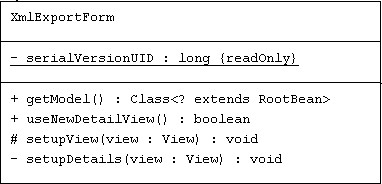
\includegraphics[width=0.7\textwidth]{imgs/XmlExportForm.jpg}
	\caption{Структура формы главной таблицы}
	\label{fig:form}
\end{figure}

Описание методов.

\begin{itemize}
    \item \textit{serialVersionUID()} Это идентификатор, являющейся константой и показывающий в какой версии приложения появился интерфйес.
    \item \textit{getModel()} Это необходимый для реализации метод, связывающий класс формы с моделью данных. Ссылку на класс модели данных.
    \item \textit{setupView()} Это основной метод формы, в котором настраивается то, как на ней будут отображаться данные моделей.
    \item \textit{useNewDetailView()} Это переопределённый метод, который просто возвращает значение истина, поменять способ отображения детализаций. Этот способ наиболее подходящий для работы с инструментом, так как основная работа заключается в создании элементов структуры.
    \item \textit{setupDetails()} Служебный метод, который добавляет детализации к элементам главной таблицы.
\end{itemize}

Пункт 2 будет рассмотрен подробно далее. 

Для задания колонок используются <<биндинги>>. Это экземпляры класса GridBinding, внутреннего класса проекта, которые хранят информацию о колонках на какой-либо форме. Внутри него записываются другие внутренние классы GridAttributes, который отвечают за настройку отображения данных в конкретной колонке формы.

Для удобства <<биндинги>> формы и всех детализаций вынесены в отдельный класс, чья структура показана на рисунке \ref{fig:binding}.

\begin{figure}[h!]
	\centering
	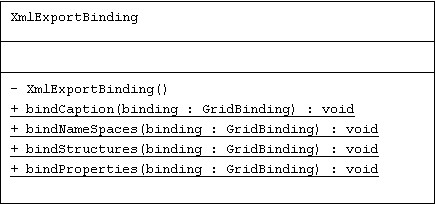
\includegraphics[width=0.9\textwidth]{imgs/XmlExportBindings.jpg}
	\caption{Структура класса-хранилища <<биндингов>> формы и детализаций}
	\label{fig:binding}
\end{figure}

\begin{itemize}
    \item \textit{bindCaption()} Хранит <<биндинг>> для формы главной таблицы.
    \item \textit{bindNameSpaces()} Хранит <<биндинг>> для детализации <<Пространства имён>>.
    \item \textit{bindStructures()} Хранит <<биндинг>> для детализации Структура
    \item \textit{bindProperties()} Хранит <<биндинг>> для детализации Атрибуты
\end{itemize}

\section{Описание и реализация служебных моделей данных инструмента}

В проекте для каждого интерфейса проекта описывается Модель данных в нём, в виде Java-интерфейса, У каждой модели обязательно должны быть определены поля \textit{TABLE\_NAME} - название таблицы и \textit{ENTITY\_NAME} -- название сущности. Они нужны Hibernate для создания представления модели в базе данных и в своих внутренних файлах. То же самое необходимо сделать и для каждой детализации.

Название главной таблицы будет <<Структура экспорта XML>>. Служебная модель данных будет \textit{XmlExportData}. Будут необходимы поля для Кода, Наименования, Источника данных, Массива пространств имён, чтобы хранить там ссылки на созданные в детализации <<Пространства имён>> и массив элементов структуры, который также нужен для хранения элементов детализации <<Структуры>>. Дополнительно задано поле \textit{CLS\_MASK}, оно нужно для того, чтобы сказать Hibernate, сколько места будет занимать Код, дабы оптимизировать способ его хранения в базе данных приложения. Структура класса показана на рисунке \ref{fig:maintable}.

\hfill

\begin{figure}[h!]
	\centering
	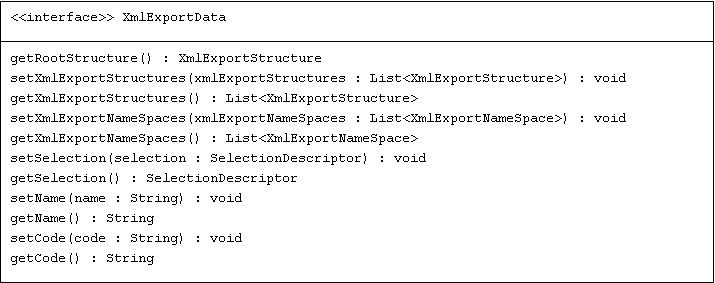
\includegraphics[width=\textwidth]{imgs/XmlExportData.jpg}
	\caption{Структура модели XmlExportData}
	\label{fig:maintable}
\end{figure}

\begin{itemize}
    \item \textit{getRootStructure()} Это вычислимое поле, которое возвращает ссылку на корневой элемент структуры элементов. Возвращает элемент, у которого не указана ссылка на предка.
    \item \textit{getXmlExportStructures() и setXmlExportStructures()} Они отвечают за поле, обращение к которому через метод \textit{get} вернёт список всех элементов структуры, созданных в соответствующей детализации. Через метод \textit{set} можно задать данный список, который после будет интерпретирован Hibernate в отношение, указанное в модели. В данном случае это OneToMany (<<Один ко многим>>).
    \item \textit{getXmlExportNameSpaces() и setXmlExportNameSpaces()} Они отвечают за поле, обращение к нему вернёт все пространства имён, которые были указаны в соответсвующей детализации. Принцип действия метода \textit{set} не отличается от такового в пункте 1.
    \item \textit{getSelection() и setSelection()} Это методы, отвечающие за хранение и изменение ссылки на источник данных.
    \item \textit{getName() и setName()} Отвечают за хранение текстового значения Наименования структуры экспорта.
    \item \textit{getCode() и setCode()} Отвечают за хранение текстового значение Кода структуры экспорта.
\end{itemize}

Модель пространства имён. Детализация будет иметь имя <<Пространство имён>>. Для неё нам будут необходимы поля для тега пространства и имени пространства. Они будут строковыми. Более подробно указано на рисунке \ref{fig:namespace}.

\begin{figure}[h!]
	\centering
	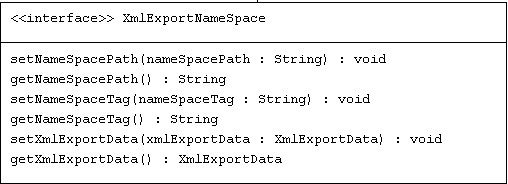
\includegraphics[width=\textwidth]{imgs/XmlExportNameSpace.jpg}
	\caption{Структура модели XmlExportNameSpace}
	\label{fig:namespace}
\end{figure}

\begin{itemize}
    \item \textit{getNameSpacePath() и setNameSpacePath()} Хранят путь к имени пространства, например \textit{http://www.w3.org/2001/XMLSchema}.
    \item \textit{getNameSpaceTag() и setNameSpaceTag()} Хранят название пространства.
    \item \textit{getXmlExportData() и setXmlExportData()} Хранят ссылку на элемент структуры экспорта.
\end{itemize}

Модель элемента структуры. Будет именоваться детализацией <<Структура>>. В нём нужны будут поля для ссылки на элемент в главной таблице, чтобы при обработке был к ней лёгкий доступ, Название тега, который будет записан, Владелец, для создания вложенности, Пространство, которому тот принадлежит, Колонка источника, чтобы можно было указать какую информацию необходимо вписать и Порядок, для сортировки внутри тега. Более подробно указано на рисунке \ref{fig:struct}. 

\begin{figure}[h!]
	\centering
	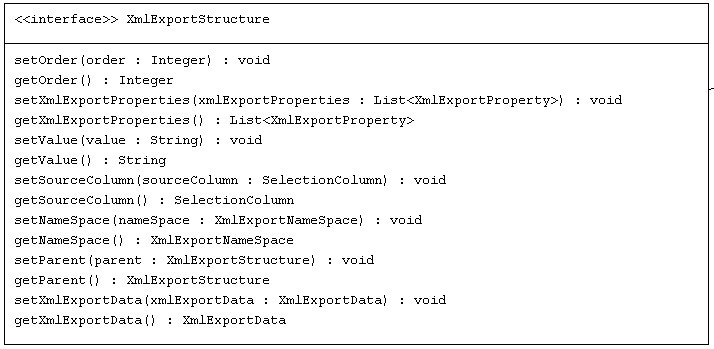
\includegraphics[width=\textwidth]{imgs/XmlExportStructure.jpg}
	\caption{Структура модели XmlExportStructure}
	\label{fig:struct}
\end{figure}

\begin{itemize}
    \item \textit{getOrder() и setOrder()} Отвечают за хранение порядка элемента.
    \item \textit{getXmlExportProperties() и setXmlExportProperties()} При вызове данных методов, соответственно, получается и изменяется таблица ссылок на атрибуты элемента.\item \textit{getValue() и setValue()} Отвечают за хранение скрипта формирования фиксированного значения элемента
    \item \textit{getSourceColumn() и setSourceColumn()} Отвечают за хранение информации о колонке, данные из которой будут в узле.
    \item \textit{getNameSpace() и setNameSpace()} Хранят ссылку на пространство имён, которому принадлежит элемент.
    \item \textit{getParent() и setParent()} Хранят ссылку элемент структуры, являющийся родительским для данного.
    \item \textit{getXmlExportData() и setXmlExportData()} Хранят ссылку на элемент структуры экспорта.
\end{itemize}

Далее сервлет. Ему необходимо хранить только сессию, для получения экземпляра модели данных и менеджер источников данных, ещё один служебный класс. Он служит для получения данных из источников. Структура приведена на рисунке \ref{fig:servletStruct}.

\begin{figure}[h!]
	\centering
	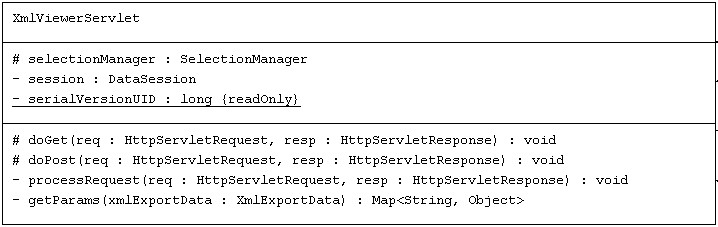
\includegraphics[width=\textwidth]{imgs/XmlViewerServlet.png.jpg}
	\caption{Структура класса XmlViewerServlet}
	\label{fig:servletStruct}
\end{figure}

\begin{itemize}
    \item \textit{session} Хранит сессию работы с базой данных. Нужна она для получения XmlExportData
    \item \textit{serialVersionUID} Хранит версию, в которой появился класс.
    \item \textit{selectionManager} Хранит ссылку на экземпляр менеджера источников данных.
    \item \textit{doGet(HttpServletRequest req, HttpServletResponse resp)} Отвечает за взаимодействия с сервлетом при GET-запросе.
    \item \textit{doPost(HttpServletRequest req, HttpServletResponse resp)} Отвечает за взаимодействия с сервлетом при POST-запросе.
    \item \textit{processRequest(HttpServletRequest req, HttpServletResponse resp)} Отвечает за выполнение запроса. Методы \textit{doPost} и \textit{doGet} вызывают его.
\end{itemize} 

На рисунке \ref{fig:interactionServl} приведена диаграмма взаимодействия с сервлетом. При GET и POST запросах она выглядит одинаково, за исключением названия метода.

\begin{figure}[h!]
	\centering
	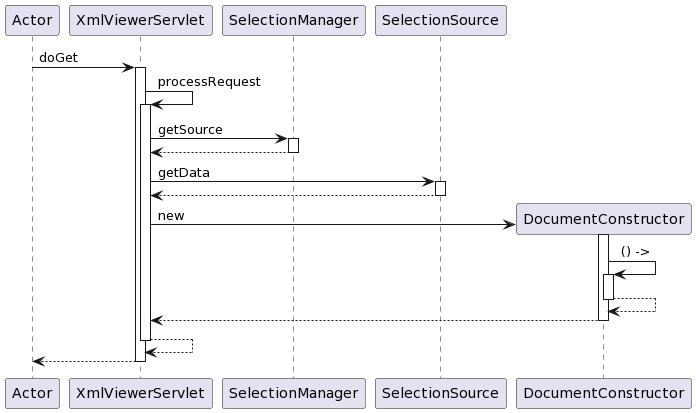
\includegraphics[width=\textwidth]{imgs/usingservlet.png}
	\caption{Диаграмма взаимодействия с сервлетом с помощью GET-запроса}
	\label{fig:interactionServl}
\end{figure}

Изначально, при вызове метода \textit{doGet}, он вызывает метод \textit{processRequest}, как и \textit{doPost}. С помощью \textit{SelectionManager}, менеджера источников данных, которые предоставляет методы работы с ними, получается сам источник методом \textit{getSource} и из него получается набор данных с помощью метода \textit{getData}. Набора дынных далее передаётся в конструктор класса \textit{DocumentConstructor}.

\section{Выбор подхода обработки XML-документа}

В Java есть три самых популярных подхода к обработке XML-документа - DOM, SAX и StAX.

DOM (Document Object Model) - это способ представление XML файла как дерево узлов. Для работы с ним необходимо создавать объект для каждого элемента документа. Это позволяет легко находить и модифицировать элементы, но в то же время требует значительно больших затрат памяти при обработке больших XML-документов.

SAX (Simple API for XML) и StAX (Streaming API for XML) похожи. При записи в файл они не требуют загрузки всей структуры в память, а работают последовательно. Из-за этого они хорошо подходят для генерации больших XML-файлов. 

Для записи в XML-файл будет использован XMLStreamWriter. Он реализует API StAX (Streaming API for XML) и удобен в работе. В сравнении с DOM нет необходимости для, например, атрибута создавать элементы как объекты, достаточно вызвать метод \textit{writeStartElement}, который создаст начальный тег (<Название тега>), записать данные с помощью \textit{writeCharacters} и закрыть тег с помощью \textit{writeEndElement}. Конечно, данный способ менее репрезентативен, нежели DOM. Тем не менее отличается хорошей производительностью при работе с большими файлами. 

В нашем случае, мы не можем точно знать количество записей в наборе данных. Если, например, необходимо экспортировать все организации из проекта в XML, то данная операция займёт кратно меньший объём памяти и не будет тратить процессорное время на создание объекта, что заметно сократит время работы.

\section{Реализация логики генерации XML-документа}

В базовом виде логика следующая:

\begin{itemize}
    \item Получить записи для экспорта
    \item Создать главный тег
    \item Построить структуру вложенности тегов
    \item Для каждого потомка главного тега
        \begin{itemize}
            \item Если у потомка и всех его потомков (в т.ч. потомков-потомков, потомков-потомков-потомков т.д.) нет элементов, использующих данные из набора данных, то создать такой элемент, используя данные из фиксированного значения.
            \item Иначе, начать рекурсивное создание элемента.
        \end{itemize}
\end{itemize}

Рекурсивное создание элемента реализовано следующим образом

\begin{itemize}
    \item Для каждой строки данных
        \begin{itemize}
            \item Получить список потомков проверяемого элемента
            \item Если у список потомков не пуст, то
                \begin{itemize}
                    \item Создать открывающую часть элемента, записать все атрибуты элемента
                    \item Отсортировать потомков по возрастанию порядка
                    \item Создать новый список данных, состоящий из одной, ныне обрабатываемой строки
                    \item Для каждого потомка из отсортированного списка вызвать метод создания элемента от самого потомка, используя как набор данных созданный на предыдущем шаге список
                    \item Создать закрывающую часть обрабатываемого элемента
                \end{itemize}
            \item Иначе
                \begin{itemize}
                    \item Если задана колонка источника данных, то получить по этой колонке данные из элемента набора данных (данных одного элемента). Иначе вычислить значение скрипта.
                    \item Если на предыдущем шаге не были получены данные или были получены пустые данные, то завершить обработку
                    \item Иначе, создать открывающую часть элемента, записать все атрибуты элемента и заполнить элемент полученным значением
                \end{itemize}
        \end{itemize}
\end{itemize}

\section{Реализация генерации в коде}

Сначала серверу отправляется запрос, в аргументах которого содержится ID записи на интерфейсе <<Структуры экспорта XML>>. Далее с помощью Hibernate получается запись в виде объекта по переданному ID, из неё берётся источник данных и у него вызывается метод получения набора данных. На данном этапе у нас есть объект главной таблицы и набор данных для сериализации.

Источник данных -- это внутренний инструмент проекта, который берёт все указанные в нём экземпляры модели и фильтрует их по указанному внутри него правилу. То есть, допустим, нужно отправить в какую-нибудь внешнюю систему все организации, у которой такой-то владелец. Источник данных в этим случае даст возможность получить разработанному инструменту нужные для сериализации данные. Более того, данный инструмент позволяет генерировать дополнительные данные, удалять пустые значения, а также группировать данные. Одним из главных его преимуществ является то, что данные для сериализации уже буду десериализованными из базы данных. То есть, если в нашей модели есть ссылка на другую и способ подгрузки её указан как <<Lazy>>, то нам не нужно будет отдельно просить Hibernate объект(ы), на которые ссылается поле. Главное достоинство этого инструмента в его сильном облегчении работы с получением данных из модели, так как результат его работы -- специальный класс, хранящий ещё массив служебных классов, внутри которых хранятся все поля модели в виде структуры. Там они представлены в виде <<Ключ--Значение>>, где ключ -- название колонки в модели, а значение -- его значение в базе данных или, в случае вычислимого поля модели, результат выполнения заданного ему вычисления. Это удобный инструмент, который часто используется в проекте в рамках других задач, поэтому будет логичным использовать его.

Далее был создан служебный класс DocumentConstructor. Он используется для выделения логики, относящейся к одному процессу инструмента. В данном случае -- процессу генерации XML-документа. В его конструктор передаётся элемент интерфейса <<Структуры экспорта XML>> и набор данных. Структура класса представлена на рисунке \ref{fig:docconstr}.

\begin{figure}[h!]
	\centering
	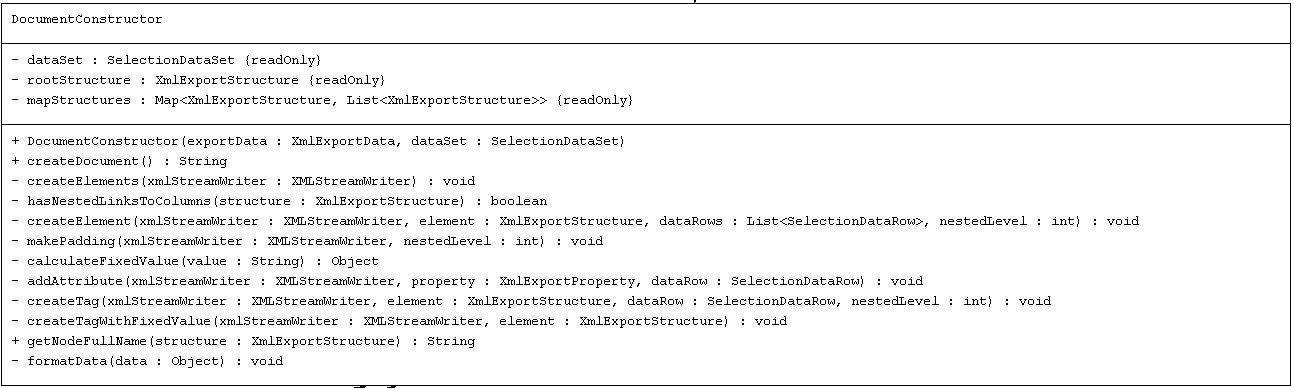
\includegraphics[width=\textwidth]{imgs/DocumentConstructor.jpg}
	\caption{Структура служебного класса DocumentConstructor}
	\label{fig:docconstr}
\end{figure}

В нём содержатся методы:

\begin{enumerate}[label=\arabic{enumi})]
    \item \textit{Map<XmlExportStructure, List<XmlExportStructure>> mapStructures} Константное поле, отвечающее за хранение структуры вложенности элементов структуры.
    \item \textit{XmlExportStructure rootStructure} Константное поле корневой структуры.
    \item \textit{SelectionDataSet dataSet} Константное поле набора данных. Представляет собой элемент внутреннего класса инструмента Источников данных, хранящий в себе набор ещё одних внутренних классов, уже представляющие удовлетворяющие фильтрам Источника данных данные.
    \item \textit{DocumentConstructor(XmlExportData exportData, SelectionDataSet dataSet)} Конструктор класса. Принимает элемент модели главной таблицы и набор данных. Он задаёт значение всех полей класса.
    \item \textit{createDocument()} Метод, создающий документ и отдающий его в виде строки.
    \item \textit{createElements(XMLStreamWriter xmlStreamWriter)} Это главный метод, из создающих элементы структуры.
    \item \textit{hasNestedLinksToColumns(XmlExportStructure structure)} Рекурсивный метод проверки наличия у элемента структуры и его потомков (в т.ч. и потомков-потомков, потомков-потомков-потомков и т.д.) заданной колонки источника данных
    \item \textit{createElement(XMLStreamWriter xmlStreamWriter, XmlExportStructure element, List<SelectionDataRow> dataRows, int nestedLevel)} Метод рекурсивного создания элемента, всех его потомков и т.д.
    \item \textit{makePadding(XMLStreamWriter xmlStreamWriter, int nestedLevel)} Метод для создания переноса на новую строчку и отступа по уровню вложенности.
    \item \textit{calculateFixedValue(String value)} Метод вычисления значения выражения на языке JavaScript, которое ему передаётся.
    \item \textit{addAttribute(XMLStreamWriter xmlStreamWriter, XmlExportProperty property, \newline
    SelectionDataRow dataRow)} Метод, добавляющий атрибут к элементу структуры.
    \item \textit{createTag(XMLStreamWriter xmlStreamWriter, XmlExportStructure element, \newline
    SelectionDataRow dataRow, int nestedLevel)} Метод создания элемента структуры (тега).
    \item \textit{createTagWithFixedValue(XMLStreamWriter xmlStreamWriter, XmlExportStructure element)} Метод создания элемента структуры с заданным значением и его атрибутов.
    \item \textit{createTagWithFixedValue(XMLStreamWriter xmlStreamWriter, XmlExportStructure element)} Метод для получения полного имени элемента, включающего идентификатор его пространства.
    \item \textit{getNodeFullName(XmlExportStructure structure)} Возвращает название элемента в виде строки с уже применённым пространством имён, если таковое задано для него.
    \item \textit{formatData(Object data)} Возвращает отформатированное значение, полученное из скрипта или колонки.
\end{enumerate}

Это общее описание методов вспомогательного класса.

В графическом виде данный алгоритм представлен на рисунках \ref{fig:algorithm1} (начало) и \ref{fig:algorithm2} (продолжение) как диаграмма последовательности. 

\begin{figure}[h!]
	\centering
	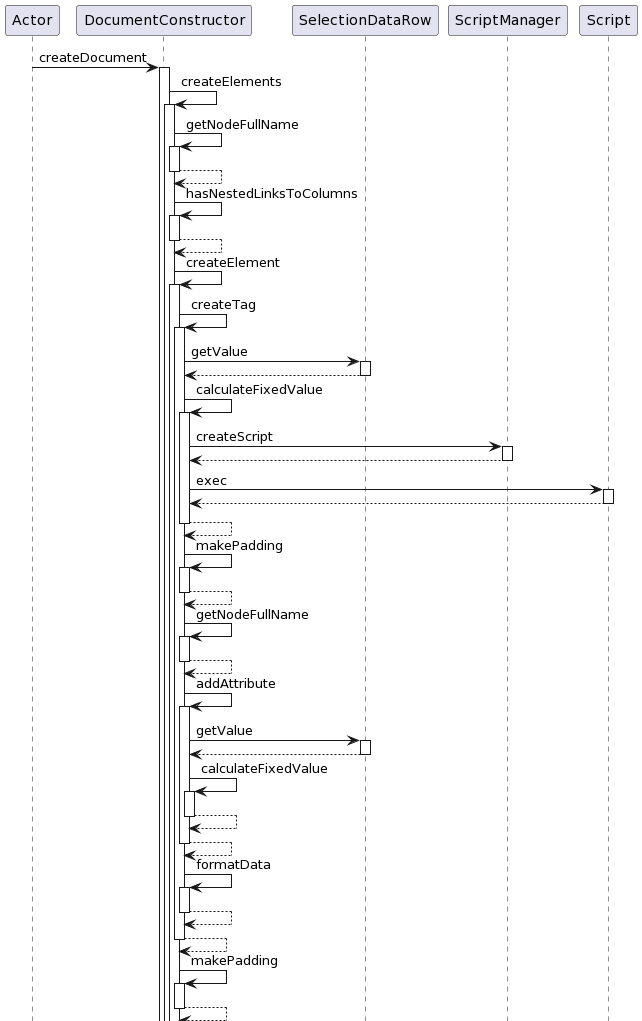
\includegraphics[width=0.9\textwidth]{imgs/crDoc1.png}
	\caption{Алгоритм генерации (начало)}
	\label{fig:algorithm1}
\end{figure}

\begin{figure}[h!]
	\centering
	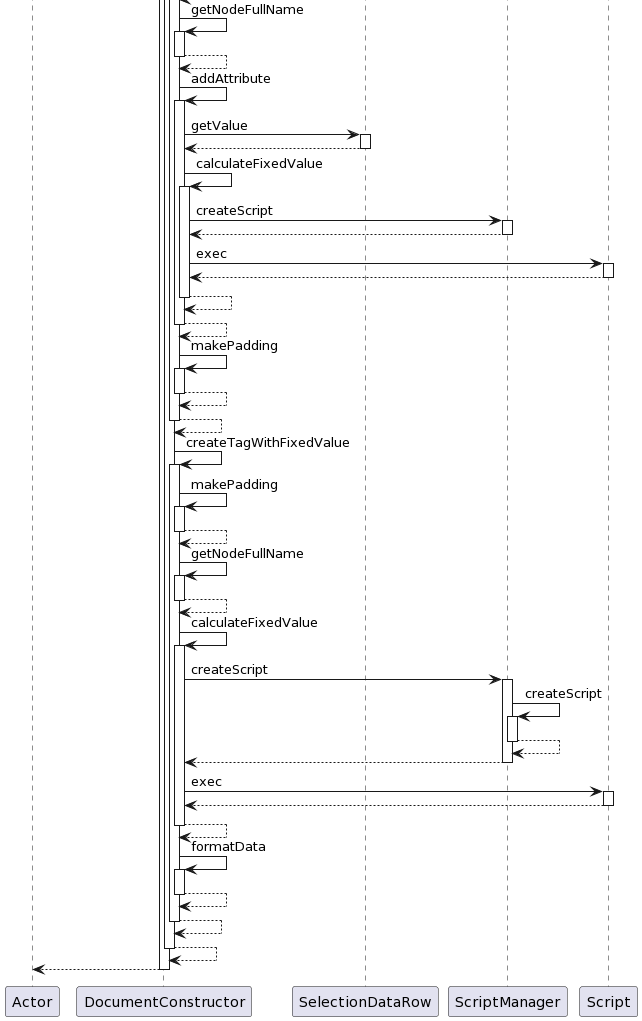
\includegraphics[width=0.9\textwidth]{imgs/crDoc2.png}
	\caption{Алгоритм генерации (продолжение)}
	\label{fig:algorithm2}
\end{figure}

Опишем данную диаграмму. Для генерации документа сервлет вызывает метод \textit{createDocument}. Внутри него создаётся экземпляр класса \textit{StringWriter}, который передаётся в \textit{XMLStreamWriter}, для его работы. У документа прописывается кодировка, в нашем случае будет использована UTF-8, и версия, будет 1.0.

Далее начинается генерация элементов, вызывается метод .createElements. С помощью метода класса \textit{XMLStreamWriter } \textit{writeStartElement} создаётся корневой элемент. При этом его имя генерируется с помощью метода \textit{getNodeFullName}. После в созданный элемент записываются все пространства имён из соответствующей детализации. С помощью структуры \textit{mapStructures} получаются все потомки корневого элемента. Эта структура была инициализирована в конструкторе \textit{DocumentConstructor} через \textit{StreamAPI} с помощью группировки полей, имеющих ссылку на родительских с их потомками. Этот список потомков сортируется по возрастанию значения порядка. 

Далее, для каждого потомка производятся следующие действия. Происходит проверка наличия в структуре всех его потомков (т.е. потомков-потомков, потомков-потомков-потомков и т.д.) наличия заданной колонки в наборе данных с помощью метода \textit{hasNestedLinksToColumns}. Его реализация такова, что если у проверяемого элемента есть заданное название колонки, то возвращается истина, иначе получаются потомки через \textit{mapStructure} и для каждого вызывается проверка этим же методом с помощью \textit{anyMatch} метода из StreamAPI, возвращающего истину если хотя бы у одного элемента списка результат метода вернул значение истина.

Если таковых нет, то это тот случай, про который шла речь в постановке под пунктом 6. То есть, это поле, которое нужно заполнить значением скрипта. Для него вызывается рекурсивный метод \textit{createTagWithFixedValue}. Его работа такова, что, если у тега есть потомок, то добавляется отступ в nestedNum размере, создаётся начальный тег с именем через \textit{getNodeFullName} и вызывается этот же метод для всех потомков. Если у потомка нет потомков, то вычисляется значение его скрипта. Если значение пустое, создаётся исключение с ошибкой о некорректности структуры (по пункту 7). После это значение обрабатывается методом \textit{formatData} и записывается возвращённое значение. Далее элемент закрывается методом \textit{writeEndElement} и делается перевод на следующую строку.

Основное предназначение \textit{formatData} -- записывать массивы в виде тегов \textit{<Название + s><Название>Элемент массива</Название>...</Название + s>}. То есть, просто обрабатывать массивы значений.

Если элементы найдены, то вызывается рекурсивный метод \textit{createElement}. Его вызов говорит, что хотя в одном элементе используется значение из набора данных. Поэтому, в нём для каждого элемента набора данных, то есть данных уже для одного экземпляра модели, а не для нескольких, происходит получение всех его потомков через \textit{mapStructure}. Если таковые есть, то это сигнализирует нам, что данный тег только обёртка для вложенных в него. Поэтому создаём его начало, полученное через \textit{getNodeFullName}, добавляем его атрибуты, сортируем потомков по возрастанию порядка и для каждого вызываем этот же метод, но уже не от набора всех строк данных, а только от одной -- обрабатываемой. Далее делаем отступ и закрываем тег. Если потомков нет, то вызываем метод \textit{createTag}. В нём получаем значение из обрабатываемой строки данных, если оно задано, а иначе значение скрипта. Тут, если оба значения получились пустыми, то тег удаляется. Если оно есть, то создаём начало тега с именем из \textit{getNodeFullName}, заполняем атрибуты, записываем значение, которое получим из метода \textit{formatData} и закрываем тег.

\section{Пример использование инструмента}

Например, необходимо экспортировать информацию обо всех сотрудниках. На интерфейсе <<Аналитические источники данных>> создаётся запись, где указывается модель \textit{Employee}. Она соответствует модели сотрудника. В приложении \ref{B} приведён пример таковой записи.

Далее на интерфейсе <<Структура экспорта XML>> добавляется новая запись, у которой в источнике указана запись, созданная ранее. Пример таковой представлен в приложении \ref{V}. В детализацию добавляется желаемая структура. Допустим, необходимо создать структуру как показано в листинге \ref{A}. То есть, в теге \textit{Body} нужно записать идентификатор записи, а сам его сделать из пространства \textit{xs}. Внутри него создать теги \textit{Name, Surname, MiddleName, DateofBirth, INN, SNILS, Position, OrganizationId}. Также нужно создать тег \textit{CreateDateTime}, написав там дату создания документа.

После необходимо заполнить детализации <<структура>> и <<пространство имён>>. Заполнение таковых приведено на рисунке \ref{G} для <<пространство имён>> и \ref{D} для <<структура>>.

После генерации файла можем его открыть и убедиться, что данные были сформированы в соответствии с заданной структурой. Пример сгенерированного файла представлен в приложении \ref{E}.

\chapternonum{Заключение}

В ходе выполнения ВКР был разработан инструмент экспорта данных моделей в формате XML. Он позволяет сохранять информацию о моделях в одном файле, обеспечивая возможность последующей загрузки данных в любые типы приложений, поддерживающие данный формат.

Инструмент позволяет разработчикам настраивать структуру необходимого им XML-файла намного удобнее чем это могло бы быть реализовано с помощью аннотаций к моделям и полям в них. Это позволяет быстрее менять структуры, так как нет необходимости пересобирать проект. Также данный способ реализации добавляет наглядности структуре тегов в итоговом XML-файле. Если в модели есть, например, 20 полей, а информация только из 10 необходимо экспортировать, то разобраться в структуре будет достаточно сложно. Инструмент устраняет эту проблемы.

Были реализованы все пункты постановки. Функции инструмента могут быть несложным образом расширены при появлении таковой потребности. Из-за использования сервлета, как способ взаимодействия с инструментом, удалось добиться возможности вызова его из других мест проекта, что позволит пользователю получить файл удобным для него способом.

% В заключении подводятся итоги выполненной работы, рассказывается о~том, что удалось и~что не~удалось сделать, описываются перспективы продолжения исследований.
\renewcommand\bibname{Список литературы}
\bibliographystyle{ugost2003}
\bibliography{bibliography}

% Приложения
\appendix

% Настраиваем общее для всех языков оформление листинга
\lstset{
	%	breaklines=true,
	%	frame=l,
	%	showstringspaces=false,
	tabsize=4, % длина табуляции в пробелах
	formfeed=\newpage, % реакция на символ "form feed"
	extendedchars=true, % используем неанглийские буквы
	basicstyle=\ttfamily, % базовый стиль
%	keywordstyle=\bfseries, % стиль ключевых слов (попробуйте \pmb если \bfseries не работает)
	commentstyle=\rmfamily\itshape, % стиль для комментариев
	stringstyle=\slshape, % стиль строк в кавычках
	numbers=left, % где проставляем номера строк; возможные значения: none, left, right
	numbersep=1em, % расстояние (по горизонтали) от номеров строк до кода
	stepnumber=1, % шаг отображения номеров строк. Если 1, то каждая строка помечается номером
	numberstyle=\footnotesize\color{black}, % стиль для номеров строк
}

\chapter{Пример структуры XML-файла}
\label{A}

\lstset{frame=tb,
  aboveskip=3mm,
  belowskip=3mm,
  showstringspaces=false,
  columns=flexible,
  basicstyle={\small\ttfamily},
  numbers=left,
  numberstyle=\tiny\color{gray},
  keywordstyle=\color{blue},
  commentstyle=\color{dkgreen},
  stringstyle=\color{black},
  breaklines=true,
  breakatwhitespace=true,
  tabsize=3
}

\lstdefinestyle{XML}{
  language=XML,
  morekeywords={text,id},
}

\begin{lstlisting}[style=XML,  label=lst:aggregationBinding]
<Employee xmlns:xs="http://www.w3.org/2001/XMLSchema">
  <xs:Body id="...">
    <Name>...</Name>
    <Surname>...</Surname>
    <MiddleName>...</MiddleName>
    <INN>...</INN>
    <SNILS>...</SNILS>
    <Position>...</Position>
    <OrganizationId>...</OrganizationId>
  </xs:Body>
  <xs:Body id="...">
    <Name>...</Name>
    <Surname>...</Surname>
    <MiddleName>...</MiddleName>
    <INN>...</INN>
    <SNILS>...</SNILS>
    <Position>...</Position>
    <OrganizationId>...</OrganizationId>
  </xs:Body>
  ...
  <CreateDateTime>...</CreateDateTime>
</Employee>
\end{lstlisting}

\chapter{Пример источника данных}
\label{B}

\begin{figure}[!ht]
	\centering
	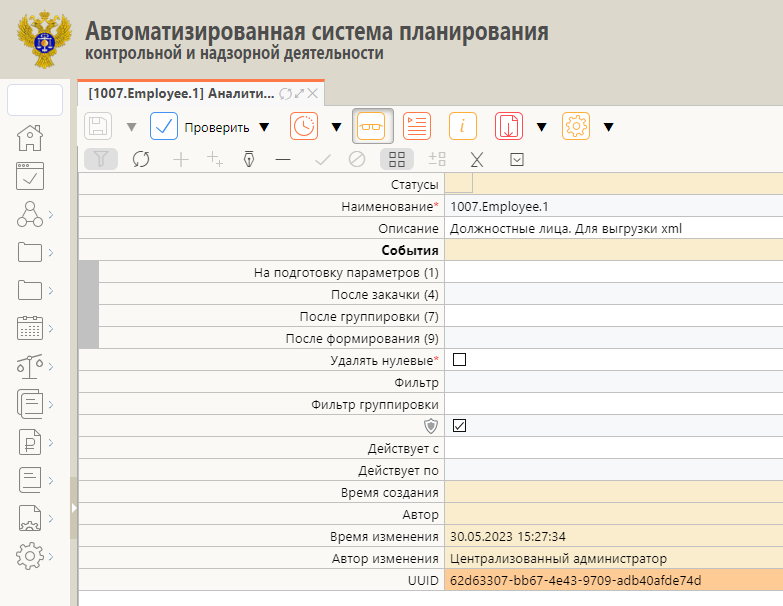
\includegraphics[width=\textwidth]{imgs/source.png}
	\label{fig:0} % Метка для ссылки в тексте
\end{figure}

\chapter{Пример записи в главной таблице}
\label{V}

\begin{figure}[!ht]
	\centering
	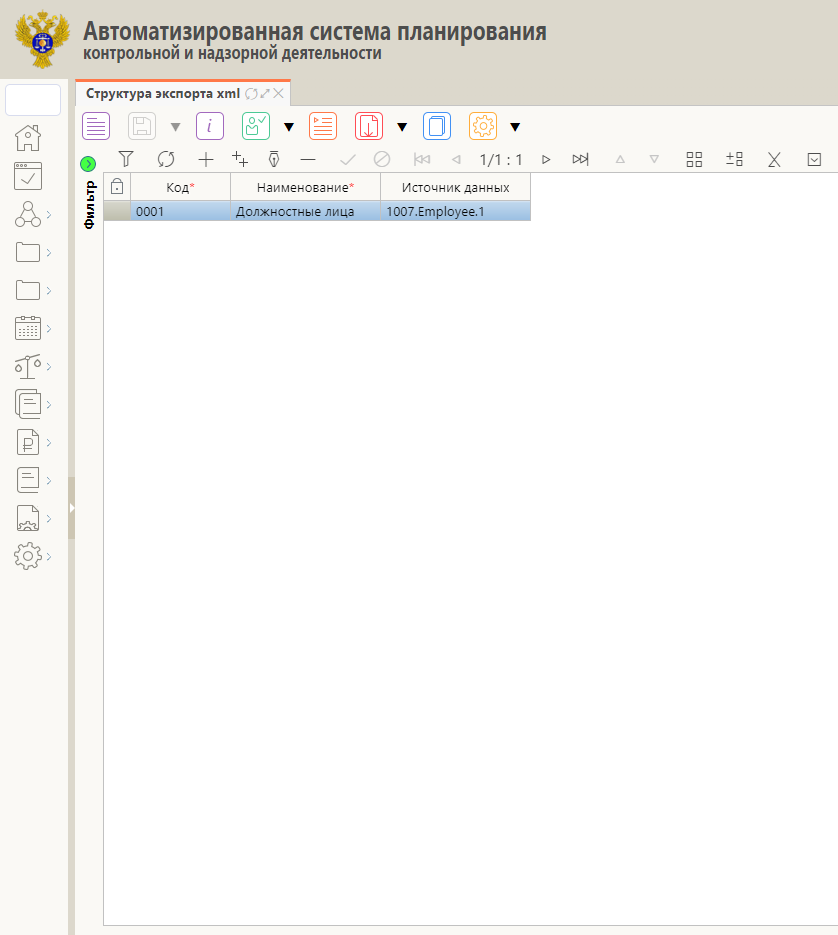
\includegraphics[width=\textwidth]{imgs/main.png}
	\label{fig:1} % Метка для ссылки в тексте
\end{figure}

\chapter{Интерфейс таблицы <<Имя пространства>>}
\label{G}

\begin{figure}[!ht]
	\centering
	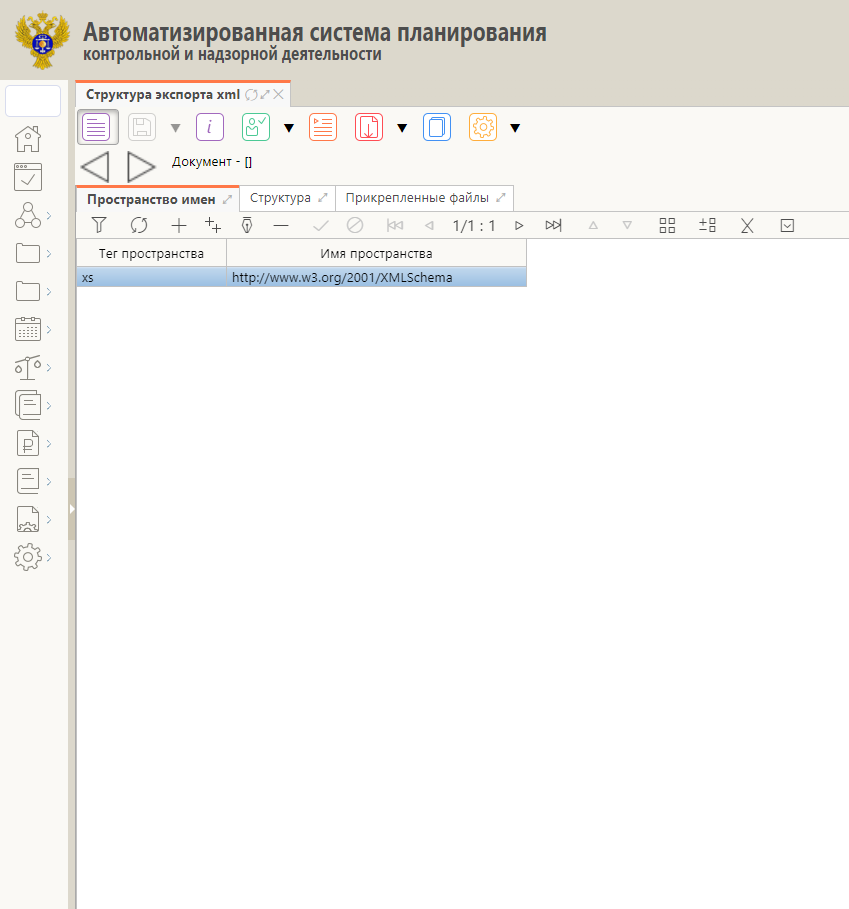
\includegraphics[width=\textwidth]{imgs/Namespaces.png}
	\label{fig:2} % Метка для ссылки в тексте
\end{figure}

\chapter{Интерфейс таблицы <<Структура>>}
\label{D}

\begin{figure}[!ht]
	\centering
	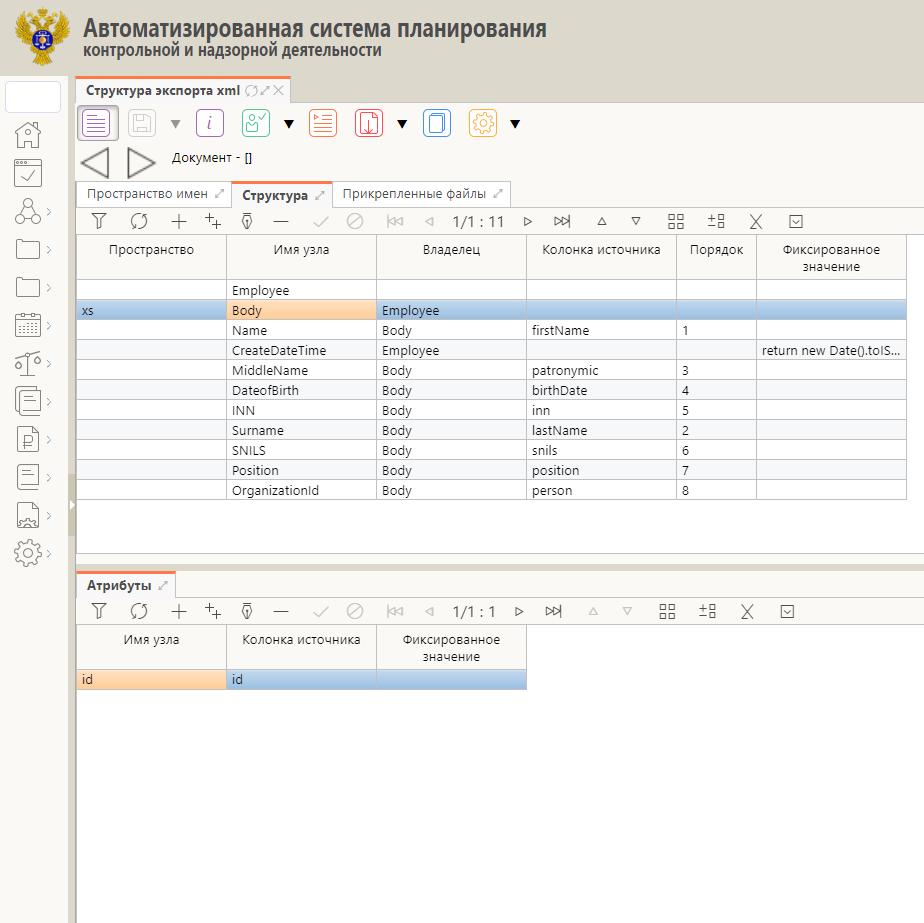
\includegraphics[width=\textwidth]{imgs/struct.png}
	\label{fig:3} % Метка для ссылки в тексте
\end{figure}

\chapter{Пример сгенерированного по структуре из приложения \ref{D} документа}
\label{E}

\lstset{frame=tb,
  aboveskip=3mm,
  belowskip=3mm,
  showstringspaces=false,
  columns=flexible,
  basicstyle={\small\ttfamily},
  numbers=left,
  numberstyle=\tiny\color{gray},
  keywordstyle=\color{blue},
  commentstyle=\color{dkgreen},
  stringstyle=\color{black},
  breaklines=true,
  breakatwhitespace=true,
  tabsize=3,
  extendedchars=false
}

\lstdefinestyle{XML}{
  language=XML,
  morekeywords={text,id},
}

\
\begin{lstlisting}[style=XML,  label=lst:aggregationBinding]
<?xml version='1.0' encoding='UTF-8'?>
<Employee xmlns:xs="http://www.w3.org/2001/XMLSchema">
  <xs:Body id="124">
    <Name>Иван</Name>
    <Surname>Иванов</Surname>
    <MiddleName>Иванович</MiddleName>
    <INN>123456789012</INN>
    <SNILS>12345678901</SNILS>
    <Position>Сотрудник</Position>
    <OrganizationId>126</OrganizationId>
  </xs:Body>
  <xs:Body id="123">
    <Name>Иван</Name>
    <Surname>Иванов</Surname>
    <MiddleName>Иванович</MiddleName>
    <INN>123456789013</INN>
    <SNILS>12345678902</SNILS>
    <OrganizationId>127</OrganizationId>
  </xs:Body>
  <CreateDateTime>2023-06-07T13:24:26.975Z</CreateDateTime>
</Employee>
\end{lstlisting}

% Конец документа
\end{document}
